% Options for packages loaded elsewhere
\PassOptionsToPackage{unicode}{hyperref}
\PassOptionsToPackage{hyphens}{url}
\PassOptionsToPackage{dvipsnames,svgnames,x11names}{xcolor}
%
\documentclass[
  9pt,
  letterpaper,
  DIV=11,
  numbers=noendperiod]{scrartcl}

\usepackage{amsmath,amssymb}
\usepackage{setspace}
\usepackage{iftex}
\ifPDFTeX
  \usepackage[T1]{fontenc}
  \usepackage[utf8]{inputenc}
  \usepackage{textcomp} % provide euro and other symbols
\else % if luatex or xetex
  \usepackage{unicode-math}
  \defaultfontfeatures{Scale=MatchLowercase}
  \defaultfontfeatures[\rmfamily]{Ligatures=TeX,Scale=1}
\fi
\usepackage{lmodern}
\ifPDFTeX\else  
    % xetex/luatex font selection
\fi
% Use upquote if available, for straight quotes in verbatim environments
\IfFileExists{upquote.sty}{\usepackage{upquote}}{}
\IfFileExists{microtype.sty}{% use microtype if available
  \usepackage[]{microtype}
  \UseMicrotypeSet[protrusion]{basicmath} % disable protrusion for tt fonts
}{}
\usepackage{xcolor}
\usepackage[lmargin=0.25in,rmargin=0.25in,tmargin=0in,bmargin=0.25in]{geometry}
\setlength{\emergencystretch}{3em} % prevent overfull lines
\setcounter{secnumdepth}{-\maxdimen} % remove section numbering
% Make \paragraph and \subparagraph free-standing
\makeatletter
\ifx\paragraph\undefined\else
  \let\oldparagraph\paragraph
  \renewcommand{\paragraph}{
    \@ifstar
      \xxxParagraphStar
      \xxxParagraphNoStar
  }
  \newcommand{\xxxParagraphStar}[1]{\oldparagraph*{#1}\mbox{}}
  \newcommand{\xxxParagraphNoStar}[1]{\oldparagraph{#1}\mbox{}}
\fi
\ifx\subparagraph\undefined\else
  \let\oldsubparagraph\subparagraph
  \renewcommand{\subparagraph}{
    \@ifstar
      \xxxSubParagraphStar
      \xxxSubParagraphNoStar
  }
  \newcommand{\xxxSubParagraphStar}[1]{\oldsubparagraph*{#1}\mbox{}}
  \newcommand{\xxxSubParagraphNoStar}[1]{\oldsubparagraph{#1}\mbox{}}
\fi
\makeatother


\providecommand{\tightlist}{%
  \setlength{\itemsep}{0pt}\setlength{\parskip}{0pt}}\usepackage{longtable,booktabs,array}
\usepackage{calc} % for calculating minipage widths
% Correct order of tables after \paragraph or \subparagraph
\usepackage{etoolbox}
\makeatletter
\patchcmd\longtable{\par}{\if@noskipsec\mbox{}\fi\par}{}{}
\makeatother
% Allow footnotes in longtable head/foot
\IfFileExists{footnotehyper.sty}{\usepackage{footnotehyper}}{\usepackage{footnote}}
\makesavenoteenv{longtable}
\usepackage{graphicx}
\makeatletter
\def\maxwidth{\ifdim\Gin@nat@width>\linewidth\linewidth\else\Gin@nat@width\fi}
\def\maxheight{\ifdim\Gin@nat@height>\textheight\textheight\else\Gin@nat@height\fi}
\makeatother
% Scale images if necessary, so that they will not overflow the page
% margins by default, and it is still possible to overwrite the defaults
% using explicit options in \includegraphics[width, height, ...]{}
\setkeys{Gin}{width=\maxwidth,height=\maxheight,keepaspectratio}
% Set default figure placement to htbp
\makeatletter
\def\fps@figure{htbp}
\makeatother
% definitions for citeproc citations
\NewDocumentCommand\citeproctext{}{}
\NewDocumentCommand\citeproc{mm}{%
  \begingroup\def\citeproctext{#2}\cite{#1}\endgroup}
\makeatletter
 % allow citations to break across lines
 \let\@cite@ofmt\@firstofone
 % avoid brackets around text for \cite:
 \def\@biblabel#1{}
 \def\@cite#1#2{{#1\if@tempswa , #2\fi}}
\makeatother
\newlength{\cslhangindent}
\setlength{\cslhangindent}{1.5em}
\newlength{\csllabelwidth}
\setlength{\csllabelwidth}{3em}
\newenvironment{CSLReferences}[2] % #1 hanging-indent, #2 entry-spacing
 {\begin{list}{}{%
  \setlength{\itemindent}{0pt}
  \setlength{\leftmargin}{0pt}
  \setlength{\parsep}{0pt}
  % turn on hanging indent if param 1 is 1
  \ifodd #1
   \setlength{\leftmargin}{\cslhangindent}
   \setlength{\itemindent}{-1\cslhangindent}
  \fi
  % set entry spacing
  \setlength{\itemsep}{#2\baselineskip}}}
 {\end{list}}
\usepackage{calc}
\newcommand{\CSLBlock}[1]{\hfill\break\parbox[t]{\linewidth}{\strut\ignorespaces#1\strut}}
\newcommand{\CSLLeftMargin}[1]{\parbox[t]{\csllabelwidth}{\strut#1\strut}}
\newcommand{\CSLRightInline}[1]{\parbox[t]{\linewidth - \csllabelwidth}{\strut#1\strut}}
\newcommand{\CSLIndent}[1]{\hspace{\cslhangindent}#1}

\usepackage[pages=some]{background}
% \usepackage{blindtext}
\usepackage[fontsize=8.5pt]{fontsize}

\RedeclareSectionCommand[font=\centering\large]{section}
\RedeclareSectionCommand[
  runin=false,
  afterindent=false,
  font = \normalfont\textbf,
  beforeskip=1pt,
  afterskip=1pt]{subsection}

\setlength{\itemsep}{1pt}
\setlength{\parskip}{0pt}
\setlength{\parsep}{0pt}
\setlength{\labelsep}{0pt}
\setlength{\topsep}{0pt}
\setlength{\parsep}{0pt}
\setlength{\partopsep}{0pt}
\usepackage{fontspec}
\usepackage{multirow}
\usepackage{multicol}
\usepackage{colortbl}
\usepackage{hhline}
\newlength\Oldarrayrulewidth
\newlength\Oldtabcolsep
\usepackage{longtable}
\usepackage{array}
\usepackage{hyperref}
\usepackage{float}
\usepackage{wrapfig}
\KOMAoption{captions}{tableheading}
\makeatletter
\@ifpackageloaded{caption}{}{\usepackage{caption}}
\AtBeginDocument{%
\ifdefined\contentsname
  \renewcommand*\contentsname{Table of contents}
\else
  \newcommand\contentsname{Table of contents}
\fi
\ifdefined\listfigurename
  \renewcommand*\listfigurename{List of Figures}
\else
  \newcommand\listfigurename{List of Figures}
\fi
\ifdefined\listtablename
  \renewcommand*\listtablename{List of Tables}
\else
  \newcommand\listtablename{List of Tables}
\fi
\ifdefined\figurename
  \renewcommand*\figurename{Figure}
\else
  \newcommand\figurename{Figure}
\fi
\ifdefined\tablename
  \renewcommand*\tablename{Table}
\else
  \newcommand\tablename{Table}
\fi
}
\@ifpackageloaded{float}{}{\usepackage{float}}
\floatstyle{ruled}
\@ifundefined{c@chapter}{\newfloat{codelisting}{h}{lop}}{\newfloat{codelisting}{h}{lop}[chapter]}
\floatname{codelisting}{Listing}
\newcommand*\listoflistings{\listof{codelisting}{List of Listings}}
\makeatother
\makeatletter
\makeatother
\makeatletter
\@ifpackageloaded{caption}{}{\usepackage{caption}}
\@ifpackageloaded{subcaption}{}{\usepackage{subcaption}}
\makeatother

\ifLuaTeX
  \usepackage{selnolig}  % disable illegal ligatures
\fi
\usepackage{bookmark}

\IfFileExists{xurl.sty}{\usepackage{xurl}}{} % add URL line breaks if available
\urlstyle{same} % disable monospaced font for URLs
\hypersetup{
  pdftitle={Longfin Inshore Squid () Snapshot Ecosystem \& Socioeconomic Profile (ESP)},
  colorlinks=true,
  linkcolor={blue},
  filecolor={Maroon},
  citecolor={Blue},
  urlcolor={Blue},
  pdfcreator={LaTeX via pandoc}}


\title{Longfin Inshore Squid (\protect\textit{Doryteuthis pealeii})
\linebreak Snapshot Ecosystem \& Socioeconomic Profile (ESP)}
\author{}
\date{}

\begin{document}
\maketitle


\setstretch{1}
\backgroundsetup{
  scale=1,
  angle=0,
  opacity=0,
  contents={
\includegraphics[width=\paperwidth,height=\paperheight]{bg_pg1.jpg}}
 }
\BgThispage

\vspace{-2.0cm}
\section{Spring 2026}

\begin{figure}

\begin{minipage}{0.57\linewidth}

\raggedright
\section{Key Findings from the Life History Working Group}

\subsection{Lifespan and aging}

Some literature sources estimate growth to be 1 statolith ring/day, and
literature review supports a lifespan of less than 1 year. Participants
at the longfin squid summit estimated a maximum age of 15 months. SQUIBS
statolith aging (2024) indicates maximum ages of 7 months for females
and 8.6 months for males (right) from squid caught in the fishery.

\vspace{0.25cm}

\subsection{Maturity (from SQUIBS)}

For squid caught in 2024, most stage 4 squid were caught in summer and
very few the rest of the year. The majority of stage 1 squid were caught
in the second half of 2024. Of 912 squid assessed, the dominant maturity
stage in females increases from fall to spring. The highest percentage
of mature male squid were caught in spring and summer.

\vspace{0.25cm}

\subsection{Migration and movement dynamics}

In November/December, longfin migrate from the inshore shelf to deep,
warm slope waters to overwinter. By May/June of the next year, they
migrate back to shallow coastal shelf waters to spawn {[}1{]}. The
fishery follows this pattern, occurring offshore in winter and inshore
in summer. Recent work hypothesizes a winter cohort that hatches south
of Cape Hatteras and migrates onto the Northeast shelf {[}2{]}. Fishery
observations describe a spatial gradient of 1-6 cm mantle length (ML)
squid from waters south of Hatteras through southern New England, with
the smallest squid detected further south. The Gulf Stream and warm core
rings may facilitate the recruitment transport of juvenile squid, but
potential for inputs to the population from the South and offshore are
difficult to quantify.

\vspace{0.25cm}

\subsection{Reproductive dynamics}

Spawning peaks inshore from late spring to early summer in the
Mid-Atlantic and southern New England {[}3{]} {[}1{]} with hatching in
late summer {[}4{]}. Consideration of the hypothesis of a winter cohort
spawning south of Hatteras indicates the presence of multiple cohorts
with some outside of the traditional Northeast shelf stock area, and
provides evidence of year-round spawning.

\vspace{0.25cm}

\subsection{Natural mortality}

Although natural mortality is expected to be age-dependent, lack of
accurate age data makes further study difficult. Using the equation
derived by Hamel and Cope {[}5{]}, natural mortality for longfin squid
can range from 0.36 (max. age = 15 mo.) to 0.675 (max. age = 8 mo.).
Cannibalism impacts natural mortality, but there is no available data to
quantify the amount of mortality this causes.

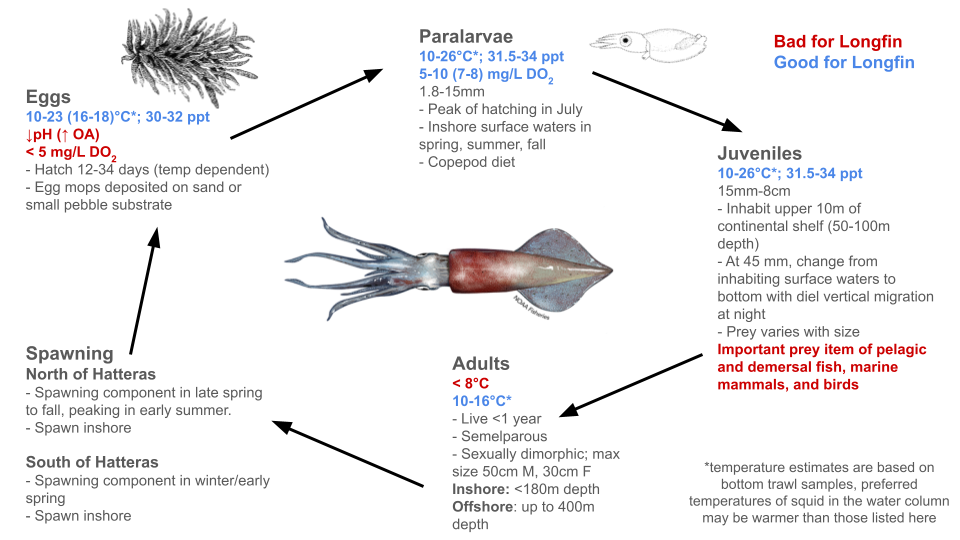
\includegraphics{C:/Users/stephanie.owen/Documents/longfinESP/images/longfin_life_history_0602.png}

\end{minipage}%
%
\begin{minipage}{0.03\linewidth}

\hfill

\end{minipage}%
%
\begin{minipage}{0.40\linewidth}

\vspace{0.50cm}
\section{Age Frequency from SQUIBS}

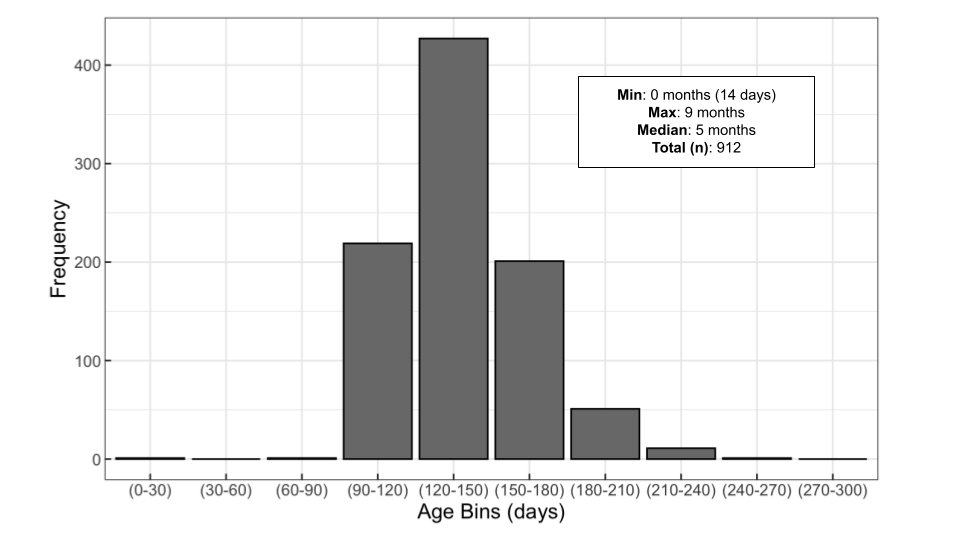
\includegraphics{C:/Users/stephanie.owen/Documents/longfinESP/images/squibs_data.png}

\section{Key Points from the Mid-Atlantic Risk Assessment}

\raggedright

The 2025 Mid-Atlantic EAFM Risk Assessment Update {[}6{]} determined
that there are moderate-high risks related to:

\begin{itemize}
\tightlist
\item
  Potential and observed distribution shifts of longfin squid
\item
  Not achieving optimum yield due to interactions with non-MAFMC managed
  species
\item
  Regulatory complexity: occasional recent changes in regulations and
  moderate (3-4) recreational regulation differences across states.
  Compliance is challenging for fishery participants given complex
  regulations.
\item
  Discards: While various management measures have minimized discards to
  the extent practicable, ecosystem changes may affect existing
  measures.
\end{itemize}

Risk elements are aspects that may threaten achieving the biological,
economic, or social objectives that the MAFMC desires from a fishery;
risk to achieving optimal yield.

Longfin squid did not score in the ``high'' risk category for any risk
elements in 2025.

\vspace{0.25cm}

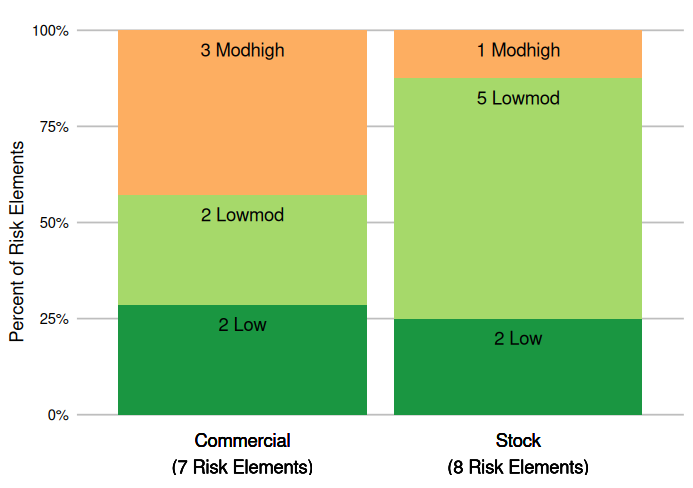
\includegraphics{C:/Users/stephanie.owen/Documents/longfinESP/images/risk_plot_new.png}

\end{minipage}%

\end{figure}%

\newpage

\backgroundsetup{
  contents={
\includegraphics[width=\paperwidth,height=\paperheight]{bg_pg2.jpg}}
  }
\BgThispage

\newgeometry{top=0.25in, left=0.25in, right=0.25in, bottom=0.25in}

\global\setlength{\Oldarrayrulewidth}{\arrayrulewidth}

\global\setlength{\Oldtabcolsep}{\tabcolsep}

\setlength{\tabcolsep}{2pt}

\renewcommand*{\arraystretch}{1.5}



\providecommand{\ascline}[3]{\noalign{\global\arrayrulewidth #1}\arrayrulecolor[HTML]{#2}\cline{#3}}

\begin{longtable*}[c]{|p{0.90in}|p{0.75in}|p{3.00in}|p{3.00in}}



\ascline{0.75pt}{666666}{1-4}

\multicolumn{1}{!{\color[HTML]{666666}\vrule width 0.75pt}>{\centering}m{\dimexpr 0.9in+0\tabcolsep}}{\textcolor[HTML]{000000}{\fontsize{10}{10}\selectfont{\global\setmainfont{Arial}{\textbf{Indicator\ Units}}}}} & \multicolumn{1}{!{\color[HTML]{666666}\vrule width 0.75pt}>{\centering}m{\dimexpr 0.75in+0\tabcolsep}}{\textcolor[HTML]{000000}{\fontsize{10}{10}\selectfont{\global\setmainfont{Arial}{\textbf{Status\ In\ 2024}}}}} & \multicolumn{1}{!{\color[HTML]{666666}\vrule width 0.75pt}>{\centering}m{\dimexpr 3in+0\tabcolsep}}{\textcolor[HTML]{000000}{\fontsize{10}{10}\selectfont{\global\setmainfont{Arial}{\textbf{Implications}}}}} & \multicolumn{1}{!{\color[HTML]{666666}\vrule width 0.75pt}>{\centering}m{\dimexpr 3in+0\tabcolsep}!{\color[HTML]{666666}\vrule width 0.75pt}}{\textcolor[HTML]{000000}{\fontsize{10}{10}\selectfont{\global\setmainfont{Arial}{\textbf{Time\ Series}}}}} \\

\ascline{0.75pt}{666666}{1-4}\endfirsthead 

\ascline{0.75pt}{666666}{1-4}

\multicolumn{1}{!{\color[HTML]{666666}\vrule width 0.75pt}>{\centering}m{\dimexpr 0.9in+0\tabcolsep}}{\textcolor[HTML]{000000}{\fontsize{10}{10}\selectfont{\global\setmainfont{Arial}{\textbf{Indicator\ Units}}}}} & \multicolumn{1}{!{\color[HTML]{666666}\vrule width 0.75pt}>{\centering}m{\dimexpr 0.75in+0\tabcolsep}}{\textcolor[HTML]{000000}{\fontsize{10}{10}\selectfont{\global\setmainfont{Arial}{\textbf{Status\ In\ 2024}}}}} & \multicolumn{1}{!{\color[HTML]{666666}\vrule width 0.75pt}>{\centering}m{\dimexpr 3in+0\tabcolsep}}{\textcolor[HTML]{000000}{\fontsize{10}{10}\selectfont{\global\setmainfont{Arial}{\textbf{Implications}}}}} & \multicolumn{1}{!{\color[HTML]{666666}\vrule width 0.75pt}>{\centering}m{\dimexpr 3in+0\tabcolsep}!{\color[HTML]{666666}\vrule width 0.75pt}}{\textcolor[HTML]{000000}{\fontsize{10}{10}\selectfont{\global\setmainfont{Arial}{\textbf{Time\ Series}}}}} \\

\ascline{0.75pt}{666666}{1-4}\endhead



\multicolumn{1}{!{\color[HTML]{666666}\vrule width 0.75pt}>{\raggedright}m{\dimexpr 0.9in+0\tabcolsep}}{\textcolor[HTML]{000000}{\fontsize{10}{10}\selectfont{\global\setmainfont{Times New Roman}{Commercial\ landings\ (millions\ of\ lbs.)
}}}\textcolor[HTML]{000000}{\fontsize{10}{10}\selectfont{\global\setmainfont{Times New Roman}{\linebreak }}}} & \multicolumn{1}{!{\color[HTML]{666666}\vrule width 0.75pt}>{\raggedright}m{\dimexpr 0.75in+0\tabcolsep}}{\textcolor[HTML]{000000}{\fontsize{10}{10}\selectfont{\global\setmainfont{Times New Roman}{Near\ long\ term\ (1996-2024)\ average}}}} & \multicolumn{1}{!{\color[HTML]{666666}\vrule width 0.75pt}>{\raggedright}m{\dimexpr 3in+0\tabcolsep}}{\textcolor[HTML]{000000}{\fontsize{10}{10}\selectfont{\global\setmainfont{Times New Roman}{Environmental\ dynamics\ vary\ between\ locations/timing\ of\ the\ summer\ and\ winter\ squid\ fisheries.\ An\ increase\ in\ landings\ since\ 2020\ but\ decrease\ in\ number\ of\ vessels\ could\ indicate\ targeted\ trips\ in\ specific\ times\ of\ year\ and\ fishers\ targeting\ other\ species\ when\ longfin\ are\ not\ available.}}}} & \multicolumn{1}{!{\color[HTML]{666666}\vrule width 0.75pt}>{\centering}m{\dimexpr 3in+0\tabcolsep}!{\color[HTML]{666666}\vrule width 0.75pt}}{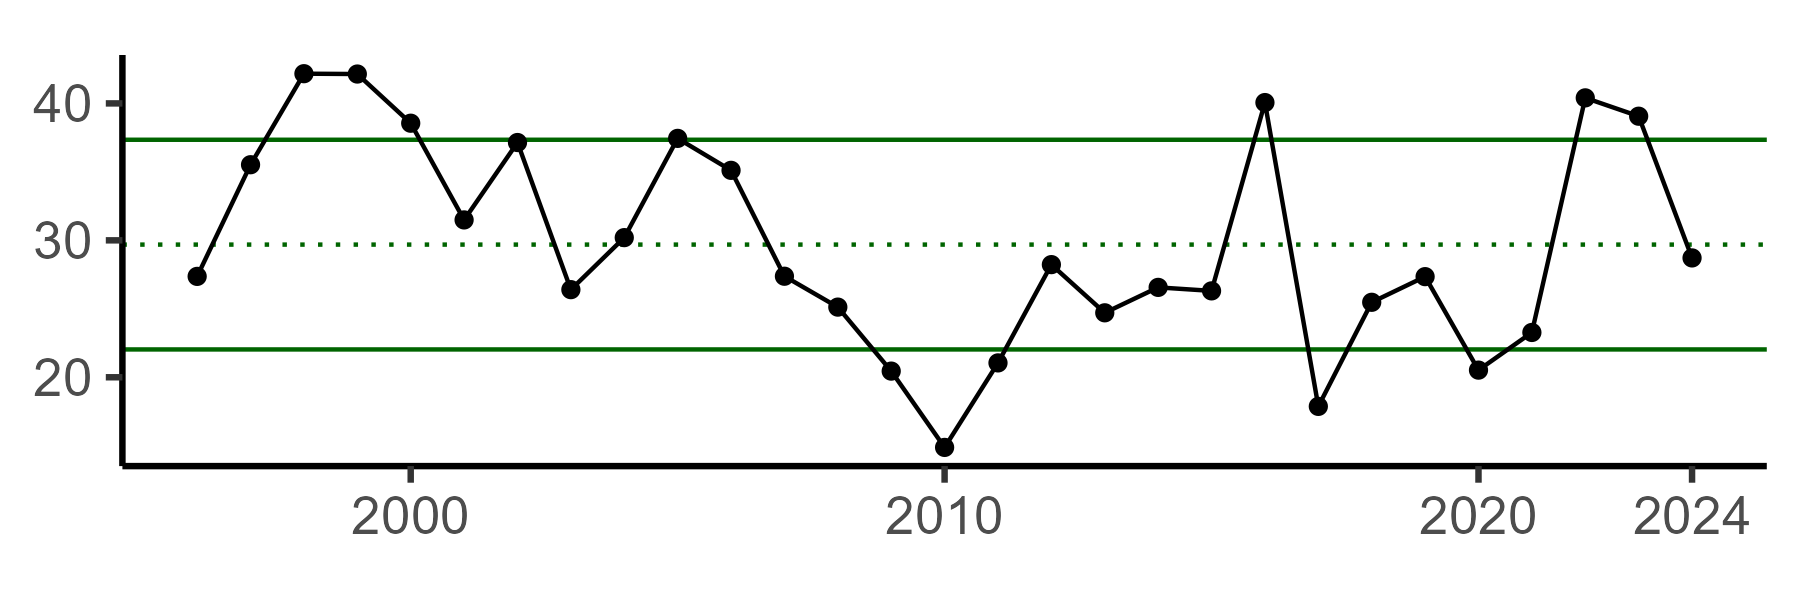
\includegraphics[width=3in, height=1in]{snapshot_template_files/figure-pdf/unnamed-chunk-2-1.png}} \\

\ascline{0.75pt}{666666}{1-4}



\multicolumn{1}{!{\color[HTML]{666666}\vrule width 0.75pt}>{\raggedright}m{\dimexpr 0.9in+0\tabcolsep}}{\textcolor[HTML]{000000}{\fontsize{10}{10}\selectfont{\global\setmainfont{Times New Roman}{Number\ of\ commercial\ vessels\ (\#\ \ of\ federally-permitted\ vessels\ landing\ over\ 1lb\ of\ longfin\ squid)}}}} & \multicolumn{1}{!{\color[HTML]{666666}\vrule width 0.75pt}>{\raggedright}m{\dimexpr 0.75in+0\tabcolsep}}{\textcolor[HTML]{000000}{\fontsize{10}{10}\selectfont{\global\setmainfont{Times New Roman}{Below\ long\ term\ (1996-2024)\ average}}}} & \multicolumn{1}{!{\color[HTML]{666666}\vrule width 0.75pt}>{\raggedright}m{\dimexpr 3in+0\tabcolsep}}{\textcolor[HTML]{000000}{\fontsize{10}{10}\selectfont{\global\setmainfont{Times New Roman}{Number\ of\ commercial\ vessels\ has\ been\ steadily
}}}\textcolor[HTML]{000000}{\fontsize{10}{10}\selectfont{\global\setmainfont{Times New Roman}{\linebreak }}}\textcolor[HTML]{000000}{\fontsize{10}{10}\selectfont{\global\setmainfont{Times New Roman}{decreasing\ since\ around\ 2000\ consistent\ with
}}}\textcolor[HTML]{000000}{\fontsize{10}{10}\selectfont{\global\setmainfont{Times New Roman}{\linebreak }}}\textcolor[HTML]{000000}{\fontsize{10}{10}\selectfont{\global\setmainfont{Times New Roman}{decreasing\ fleet\ diversity\ and\ continued\ risk\ to
}}}\textcolor[HTML]{000000}{\fontsize{10}{10}\selectfont{\global\setmainfont{Times New Roman}{\linebreak }}}\textcolor[HTML]{000000}{\fontsize{10}{10}\selectfont{\global\setmainfont{Times New Roman}{fishery\ resilience\ [7].\ Permit\ requalification\ in\ 2019\ and\ a\ decrease\ in\ the\ post-closure\ trip\ \ limit\ for\ trimester\ 2\ may\ cap\ participation,\ although\ these\ actions\ were\ designed\ to\ accommodate\ recent\ fishing\ trends\ and\ activity.}}}} & \multicolumn{1}{!{\color[HTML]{666666}\vrule width 0.75pt}>{\centering}m{\dimexpr 3in+0\tabcolsep}!{\color[HTML]{666666}\vrule width 0.75pt}}{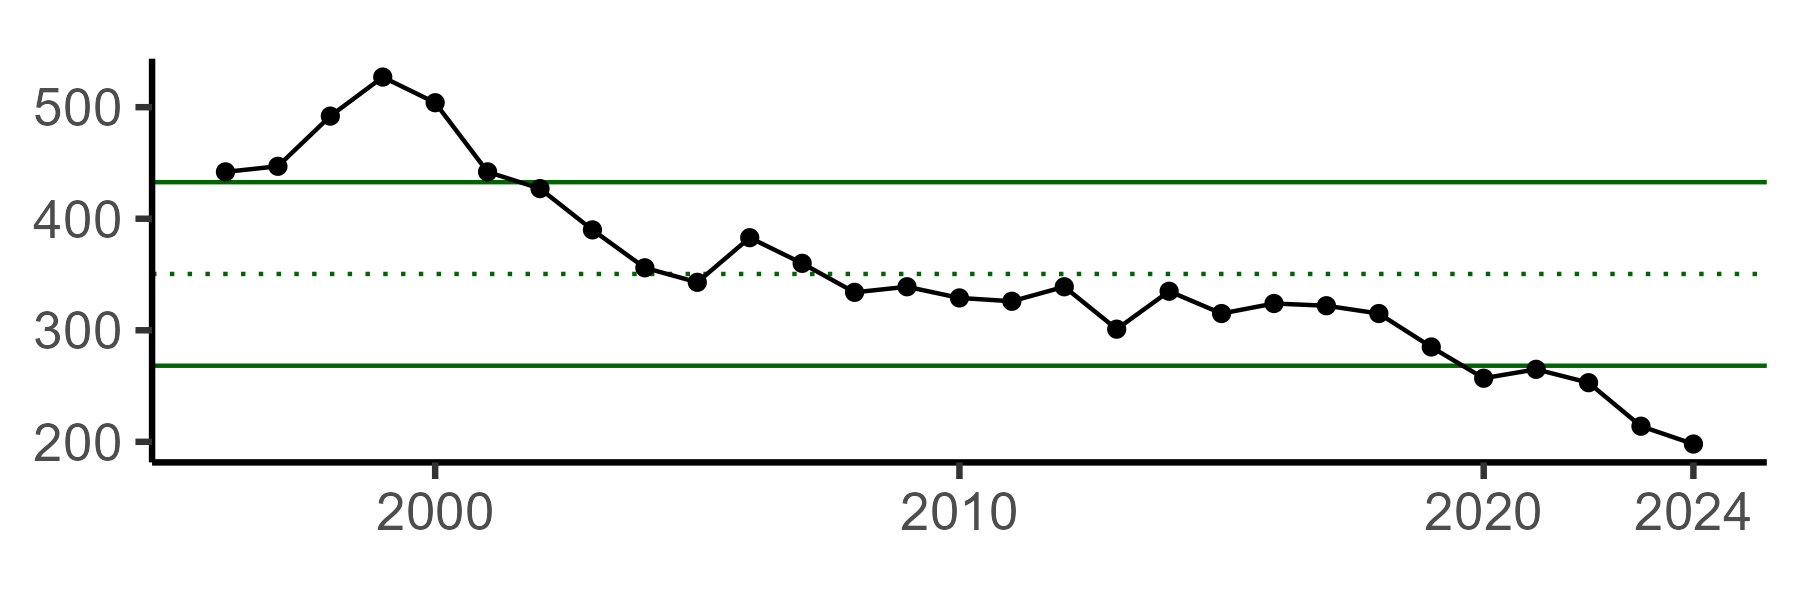
\includegraphics[width=3in, height=1in]{snapshot_template_files/figure-pdf/unnamed-chunk-2-2.png}} \\

\ascline{0.75pt}{666666}{1-4}



\multicolumn{1}{!{\color[HTML]{666666}\vrule width 0.75pt}>{\raggedright}m{\dimexpr 0.9in+0\tabcolsep}}{\textcolor[HTML]{000000}{\fontsize{10}{10}\selectfont{\global\setmainfont{Times New Roman}{Commercial\ revenue\ (millions,\ inflation\ adjusted\ to\ 2024\ USD)}}}} & \multicolumn{1}{!{\color[HTML]{666666}\vrule width 0.75pt}>{\raggedright}m{\dimexpr 0.75in+0\tabcolsep}}{\textcolor[HTML]{000000}{\fontsize{10}{10}\selectfont{\global\setmainfont{Times New Roman}{Below\ long\ term\ (1996-2024)\ average}}}} & \multicolumn{1}{!{\color[HTML]{666666}\vrule width 0.75pt}>{\raggedright}m{\dimexpr 3in+0\tabcolsep}}{\textcolor[HTML]{000000}{\fontsize{10}{10}\selectfont{\global\setmainfont{Times New Roman}{Average\ longfin\ ex-vessel\ prices\ in\ 2024
}}}\textcolor[HTML]{000000}{\fontsize{10}{10}\selectfont{\global\setmainfont{Times New Roman}{\linebreak }}}\textcolor[HTML]{000000}{\fontsize{10}{10}\selectfont{\global\setmainfont{Times New Roman}{increased\ slightly\ from\ 2023\ (+10\%),\ but
}}}\textcolor[HTML]{000000}{\fontsize{10}{10}\selectfont{\global\setmainfont{Times New Roman}{\linebreak }}}\textcolor[HTML]{000000}{\fontsize{10}{10}\selectfont{\global\setmainfont{Times New Roman}{commercial\ revenue\ has\ decreased\ from\ 2023,\ driven\ by\ the\ overall
}}}\textcolor[HTML]{000000}{\fontsize{10}{10}\selectfont{\global\setmainfont{Times New Roman}{\linebreak }}}\textcolor[HTML]{000000}{\fontsize{10}{10}\selectfont{\global\setmainfont{Times New Roman}{decrease\ in\ landings\ by\ 23\%\ [7].}}}} & \multicolumn{1}{!{\color[HTML]{666666}\vrule width 0.75pt}>{\centering}m{\dimexpr 3in+0\tabcolsep}!{\color[HTML]{666666}\vrule width 0.75pt}}{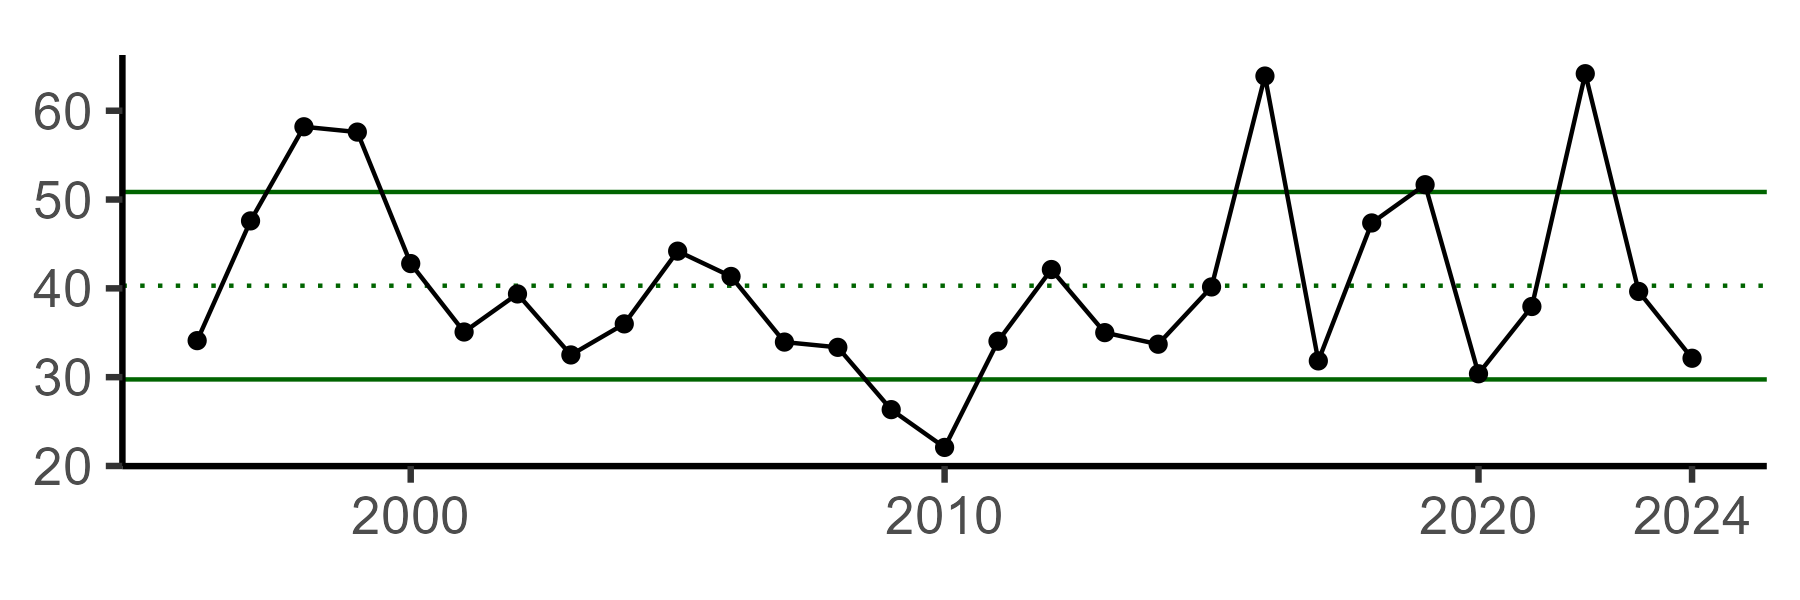
\includegraphics[width=3in, height=1in]{snapshot_template_files/figure-pdf/unnamed-chunk-2-3.png}} \\

\ascline{0.75pt}{666666}{1-4}



\multicolumn{1}{!{\color[HTML]{666666}\vrule width 0.75pt}>{\raggedright}m{\dimexpr 0.9in+0\tabcolsep}}{\textcolor[HTML]{000000}{\fontsize{10}{10}\selectfont{\global\setmainfont{Times New Roman}{Western\ Gulf\ Stream\ Index\ (shift\ in\ the\ western\ part\ of\ the\ Gulf\ Stream\ North\ wall:\ mean\ position:\ >0\ =\ more\ northerly,\ <0\ =\ more\ southerly)}}}} & \multicolumn{1}{!{\color[HTML]{666666}\vrule width 0.75pt}>{\raggedright}m{\dimexpr 0.75in+0\tabcolsep}}{\textcolor[HTML]{000000}{\fontsize{10}{10}\selectfont{\global\setmainfont{Times New Roman}{Above\ long\ term\ (1996-2024)\ average}}}} & \multicolumn{1}{!{\color[HTML]{666666}\vrule width 0.75pt}>{\raggedright}m{\dimexpr 3in+0\tabcolsep}}{\textcolor[HTML]{000000}{\fontsize{10}{10}\selectfont{\global\setmainfont{Times New Roman}{Since\ the\ mid-1990s,\ north\ and\ westward\ shifts\ in\ the\ Gulf\ Stream\ have\ resulted\ in\ an\ increase\ in\ warm\ core\ rings\ and\ deep\ water,\ high\ salinity\ heat\ waves.\ The\ position\ of\ the\ Gulf\ Stream\ influences\ seasonal\ temperature\ and\ water\ mass\ mixing\ dynamics\ that\ affect\ longfin\ squid\ habitat\ suitability,\ temperature-dependent\ growth,\ and\ prey\ availability\ (https://noaa-edab.github.io/catalog/gsi.html).}}}} & \multicolumn{1}{!{\color[HTML]{666666}\vrule width 0.75pt}>{\centering}m{\dimexpr 3in+0\tabcolsep}!{\color[HTML]{666666}\vrule width 0.75pt}}{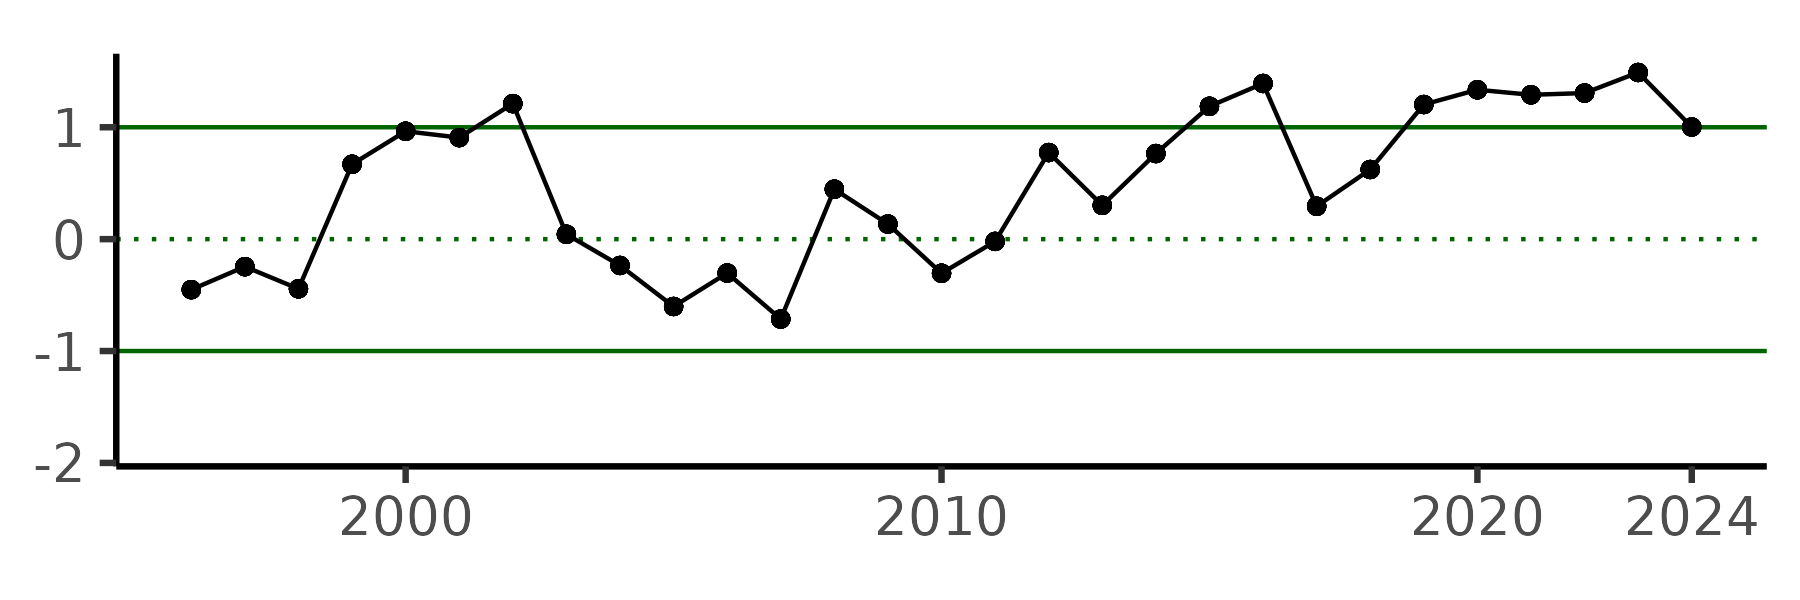
\includegraphics[width=3in, height=1in]{snapshot_template_files/figure-pdf/unnamed-chunk-2-4.png}} \\

\ascline{0.75pt}{666666}{1-4}



\multicolumn{1}{!{\color[HTML]{666666}\vrule width 0.75pt}>{\raggedright}m{\dimexpr 0.9in+0\tabcolsep}}{\textcolor[HTML]{000000}{\fontsize{10}{10}\selectfont{\global\setmainfont{Times New Roman}{Bottom\ temperature\ in\ MAB\ and\ SNE(°C)}}}} & \multicolumn{1}{!{\color[HTML]{666666}\vrule width 0.75pt}>{\raggedright}m{\dimexpr 0.75in+0\tabcolsep}}{\textcolor[HTML]{000000}{\fontsize{10}{10}\selectfont{\global\setmainfont{Times New Roman}{Above\ long\ term\ (1996-2024)\ average\ (Fall);\ near\ long\ term\ (1996-2024)\ average\ (Spring)}}}} & \multicolumn{1}{!{\color[HTML]{666666}\vrule width 0.75pt}>{\raggedright}m{\dimexpr 3in+0\tabcolsep}}{\textcolor[HTML]{000000}{\fontsize{10}{10}\selectfont{\global\setmainfont{Times New Roman}{Inshore\ temperature\ thresholds\ (around\ 14°C)\ initiate\ migration\ of\ squid\ from\ offshore\ overwintering\ habitats.\ Longfin\ squid\ seasonal\ distribution\ and\ growth\ rates\ are\ likely\ temperature\ dependent,\ avoiding\ water\ <8°C.\ Stronger\ and/or\ more\ persistent\ Mid-Atlantic\ Cold\ Pool\ conditions\ (not\ shown)\ may\ limit\ habitat\ availability\ (https://noaa-edab.github.io/catalog/cold\_pool.html).}}}} & \multicolumn{1}{!{\color[HTML]{666666}\vrule width 0.75pt}>{\centering}m{\dimexpr 3in+0\tabcolsep}!{\color[HTML]{666666}\vrule width 0.75pt}}{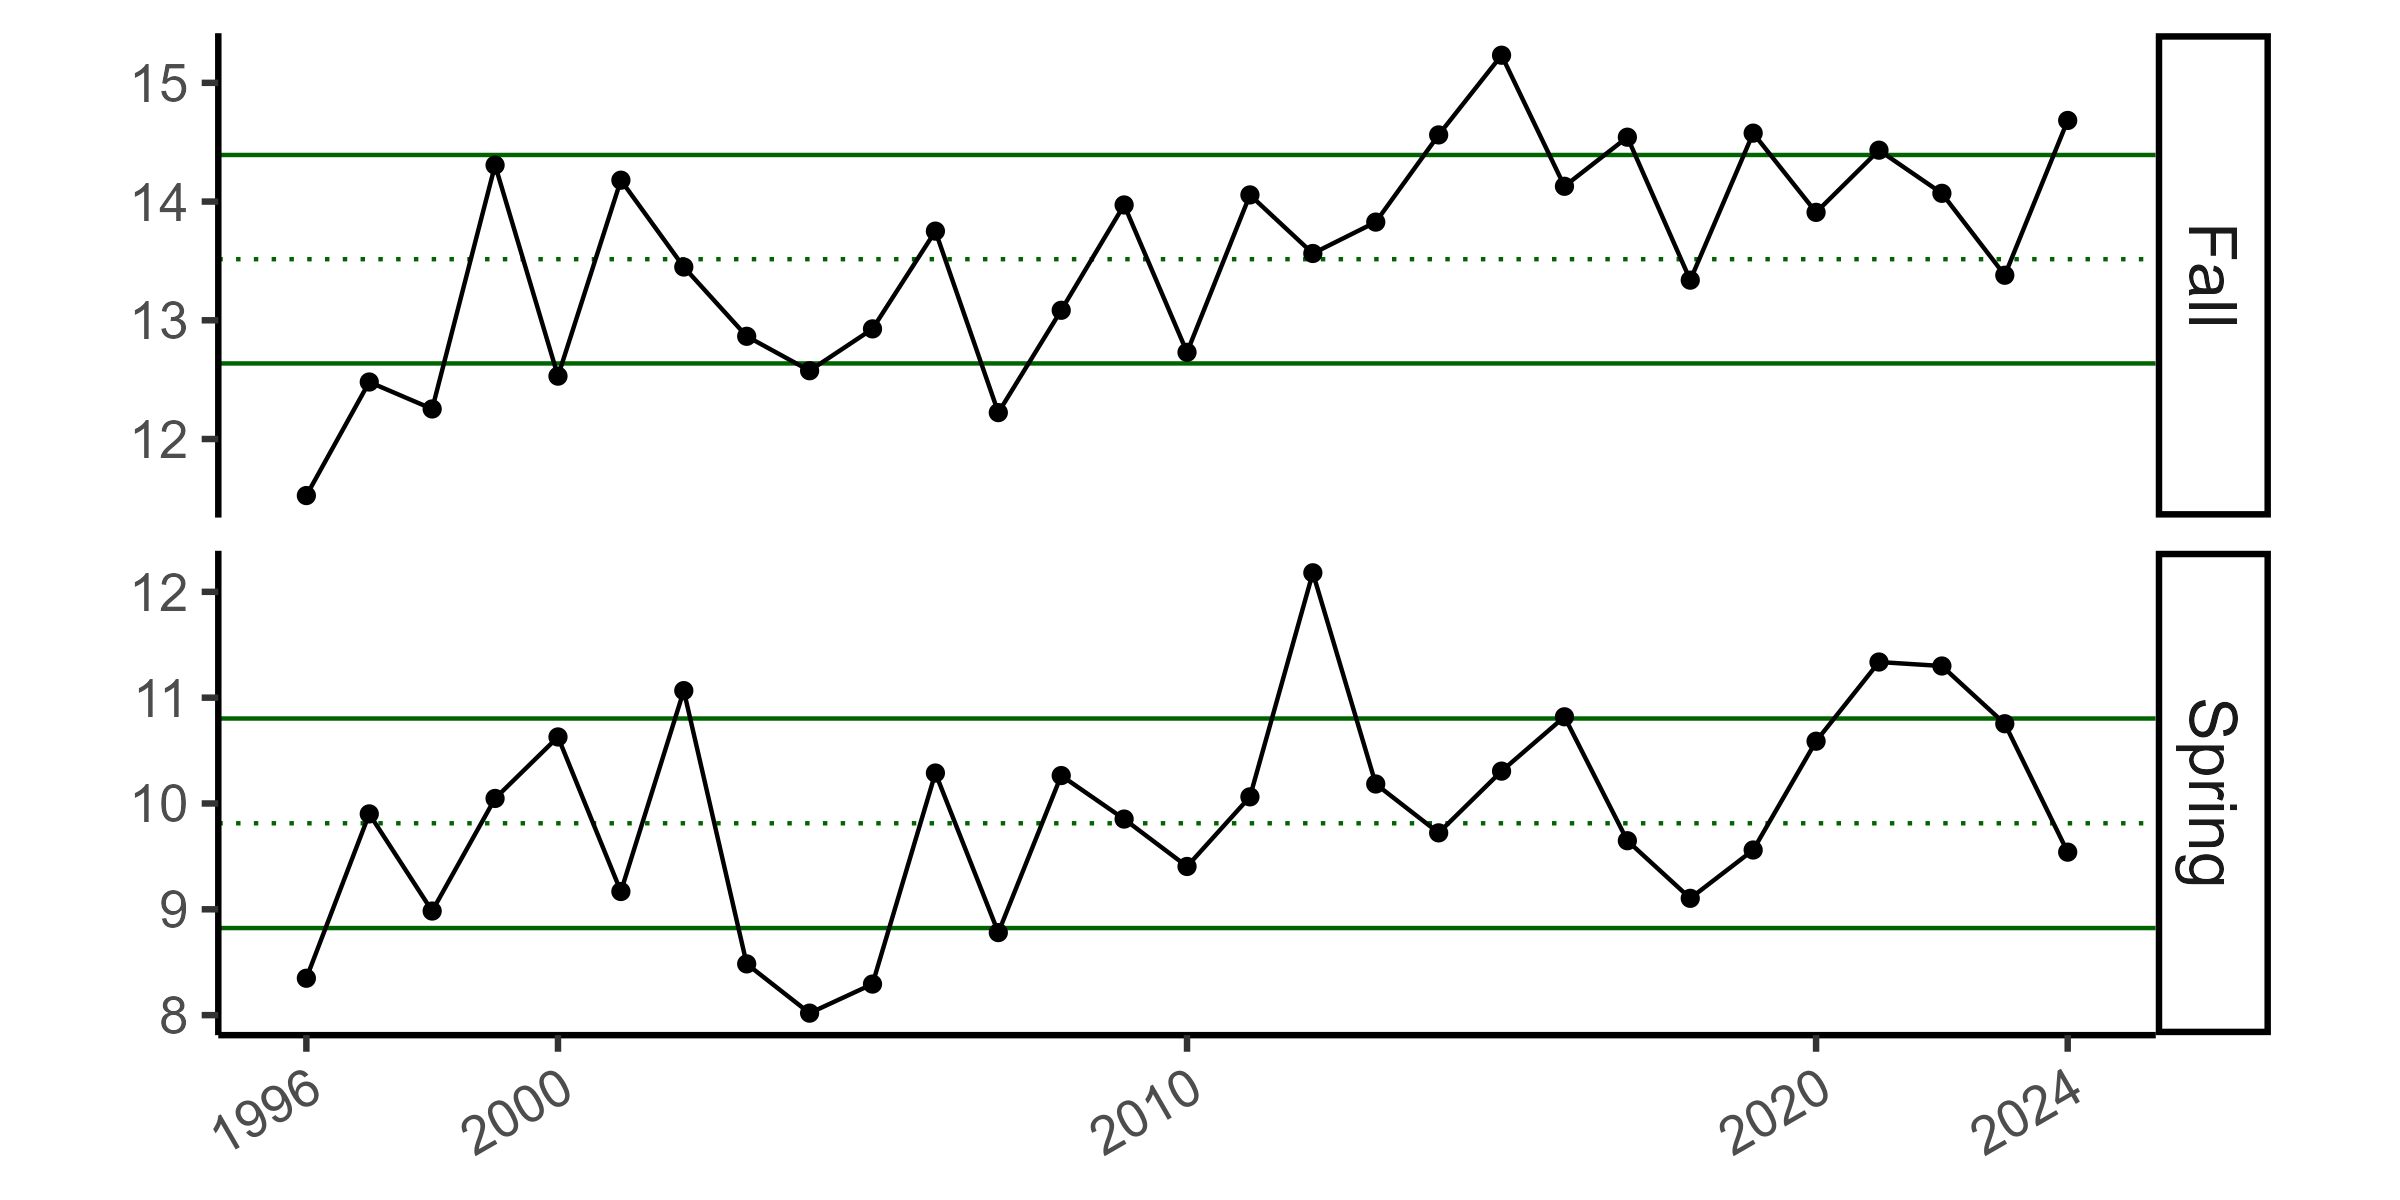
\includegraphics[width=3in, height=1.5in]{snapshot_template_files/figure-pdf/unnamed-chunk-2-5.png}} \\

\ascline{0.75pt}{666666}{1-4}



\end{longtable*}



\arrayrulecolor[HTML]{000000}

\global\setlength{\arrayrulewidth}{\Oldarrayrulewidth}

\global\setlength{\tabcolsep}{\Oldtabcolsep}

\renewcommand*{\arraystretch}{1}

\vspace{-0.4cm}

\centering\footnotesize * {[}7{]} = Longfin Squid Fishery Information
Document \newline

\normalsize\section{Data Gaps/Uncertainty}

\raggedright

\begin{itemize}
\item
  Bottom temperature data comes from GLORYS {[}8{]}, a modeled
  re-analysis product that incorporates insitu data.
\item
  The Gulf Stream Index indicator is a yearly value and may not be
  indicative of changes in oceanographic processes on a smaller time
  scale.
\item
  Aging uncertainty creates uncertainty around life history processes,
  spawning location and timing, and natural mortality.
\item
  While survey data in the 1970s and 80s indicate larval squid south of
  Cape Hatteras in the winter months that are transported north into the
  Mid-Atlantic Bight, there is a lack of definitive data to prove this
  hypothesis.
\item
  Effects of cannibalism on the population are unknown at this time.
  \vspace{0.5cm}
\end{itemize}

\centering\normalsize

We welcome your observations! Please contact
\url{northeast.ecosystem.highlights@noaa.gov} with any on-the-water
insights or changes observed in the black sea bass fishery and
\url{nefsc.esp.leads@noaa.gov} with questions or comments on the
information presented in this report.\newline

The code used to create this report can be viewed online:
\href{github.com/NEFSC/READ-EDAB/longfinESP}{github.com/NEFSC/READ-EDAB-longfinESP}

\newpage
\newgeometry{top=1in, left=1in, right=1in, bottom=1in}

\section{References}\label{references}

\phantomsection\label{refs}
\begin{CSLReferences}{0}{0}
\bibitem[\citeproctext]{ref-Macy_Brodziak_2001}
\CSLLeftMargin{1. }%
\CSLRightInline{W. Macy \& J. Brodziak, Seasonal maturity and size at
age of (\emph{{Loligo} pealeii}) in waters of southern new england.
\emph{ICES Journal of Marine Science}, \textbf{58} (2001) 852--864.
https://doi.org/\href{https://doi.org/10.1006/jmsc.2001.1076}{10.1006/jmsc.2001.1076}.}

\bibitem[\citeproctext]{ref-richardson_2026}
\CSLLeftMargin{2. }%
\CSLRightInline{D. Richardson, \emph{\href{}{A hypothesized life history
of longfin squid (\emph{{Doryteuthis} pealeii}) on the east coast of the
united states.}} (2026).}

\bibitem[\citeproctext]{ref-Hatfield_Cadrin_2002}
\CSLLeftMargin{3. }%
\CSLRightInline{E. M. C. Hatfield \& S. X. Cadrin, Geographic and
temporal patterns in size and maturity of the longfin inshore squid
(\emph{{Loligo} pealeii}) off the northeastern united states.
\emph{Fishery Bulletin}, \textbf{100} (2002) 200--213.}

\bibitem[\citeproctext]{ref-jacobson_2005}
\CSLLeftMargin{4. }%
\CSLRightInline{L. D. Jacobson,
\emph{\href{https://repository.library.noaa.gov/view/noaa/4035}{Essential
fish habitat source document. Longfin inshore squid, (\emph{{Loligo}
pealeii}), life history and habitat characteristics}} (2005).}

\bibitem[\citeproctext]{ref-Hamel_Cope_2022}
\CSLLeftMargin{5. }%
\CSLRightInline{O. S. Hamel \& J. M. Cope, Development and
considerations for application of a longevity-based prior for the
natural mortality rate. \emph{Fisheries Research}, \textbf{256} (2022)
106477.
https://doi.org/\href{https://doi.org/10.1016/j.fishres.2022.106477}{10.1016/j.fishres.2022.106477}.}

\bibitem[\citeproctext]{ref-mafmc_midatlantic_2025}
\CSLLeftMargin{6. }%
\CSLRightInline{MAFMC,
\emph{\href{https://static1.squarespace.com/static/511cdc7fe4b00307a2628ac6/t/67d45b1680e8654ecaf1b98e/1741970199497/b_Draft+MAB_RiskAssess_2025.pdf}{Mid-{Atlantic}
{EAFM} risk assessment: 2025 update}} (2025).}

\bibitem[\citeproctext]{ref-mafmc_longfin_2025}
\CSLLeftMargin{7. }%
\CSLRightInline{MAFMC,
\emph{\href{https://static1.squarespace.com/static/511cdc7fe4b00307a2628ac6/t/6806b0eab3a3986a9561ef3c/1745268972731/Longfin-FID_2025-04.pdf}{Longfin
squid (\emph{{Doryteuthis} pealeii}) fishery information document}}
(2025).}

\bibitem[\citeproctext]{ref-jeanmichel_copernicus_2021}
\CSLLeftMargin{8. }%
\CSLRightInline{L. Jean-Michel, G. Eric, B.-B. Romain, G. Gilles, M.
Angélique, D. Marie, B. Clément, H. Mathieu, L. G. Olivier, R. Charly,
C. Tony, T. Charles-Emmanuel, G. Florent, R. Giovanni, B. Mounir, D.
Yann, \& L. T. Pierre-Yves, The {Copernicus} {Global} 1/12° {Oceanic}
and {Sea} {Ice} {GLORYS12} {Reanalysis}. \emph{Frontiers in Earth
Science}, \textbf{9} (2021) 698876.
https://doi.org/\href{https://doi.org/10.3389/feart.2021.698876}{10.3389/feart.2021.698876}.}

\end{CSLReferences}




\end{document}
